
\documentclass[11pt]{article}

\usepackage{amsmath} %import amsmath for align command
\usepackage{amsfonts}
\usepackage{cite} %import package for using bibtex bibliography
\usepackage{graphicx} %import package for inserting figures from image files
\usepackage{mathtools} %import package for using certain symbols such as eq. arrows
\usepackage{tikz} %import package for creating figures
\usepackage{booktabs}
\usepackage{siunitx}
\usepackage[T1]{fontenc}
\usepackage[font=small,skip=0pt]{caption}


\usepackage{placeins}
\usepackage{array}
\newcolumntype{P}[1]{>{\centering\arraybackslash}p{#1}}

\usepackage[nodisplayskipstretch]{setspace}


\usepackage{titlesec}
\titlespacing{\section}{0pt}{0.8\baselineskip}{0.8\baselineskip}
\titlespacing{\subsection}{0pt}{0.675\baselineskip}{0.675\baselineskip}
\setlength{\abovecaptionskip}{2pt plus 2pt minus 5pt}

% for referencing links
\usepackage{hyperref}
\hypersetup{
	colorlinks=true,
	linkcolor=blue,
	filecolor=magenta,
	urlcolor=cyan,
}

% \usepackage{apacite}

\usepackage{algorithm}
\usepackage[noend]{algpseudocode}
\usepackage{textcomp}
\usepackage{subcaption}

%change default margins
\setlength{\topmargin}{-.75in}
\setlength{\textheight}{9.5in}

\setlength{\oddsidemargin}{0in}
\setlength{\evensidemargin}{0in}
\setlength{\textwidth}{6.6in}

\graphicspath{{aima/images/}}

\newcommand{\urlNewWindow}[1]{\href[pdfnewwindow=true]{#1}{\nolinkurl{#1}}}
\newcommand{\problemone}{grid world problem}
\newcommand{\Problemone}{grid world problem}
\newcommand{\problemtwo}{choice suggestion problem}
\newcommand{\Problemtwo}{choice suggestion problem}
\newcommand{\expnumber}[2]{{#1}\mathrm{e}{#2}}

\begin{document}

%create title
\title{Deep Reinforcement Learning Nanodegree\\
	   Project 2 -- Continuous Control Report}
\author{\vspace{-1mm}Chris Cadonic\\
chriscadonic@gmail.com}
\maketitle
\vspace{-1.5em}

\section{Introduction}

As part of this the deep reinforcement learning nanodegree program, this report discusses my work in training an agent to continuously control an arms that aims to reach towards a certain location that changes in 3D space over time.

\subsection{Environment Overview}

The environment, called \textit{Reacher}, is a continuous control learning condition wherein an arm is tasked to reach up to have the proximal section of the arm to remain in a specified location that may move around in 3D-space. The task of the agent is to reach up and finely adjust its positioning to continue to meet the requirements of being in this location.

For this task, the environment can be summarized as follows:

\begin{table}[!ht]
	\centering
	\begin{tabular}{ c | p{10cm} }
		\textbf{MDP property} & \textbf{characteristics} \\
		\hline
		observation space & vector of length 33, containing continuous values for position, rotation, velocity, and angular velocities \\
		\hline
		action space & vector of length 4, containing continuous values for torque to be applied to two arm joints \\
		\hline
		rewards & +0.01 for each step the agent's hand is in the target location \\
		\hline
	\end{tabular}
	\caption{Characteristics of the MDP in the Reacher environment.}
	\label{tbl:mdp}
\end{table}

\FloatBarrier

With these characteristics, the agent can learn how to maximize the amount of reward by adjusting joint torques such that it learns how to keep it's hand in the target position as often as possible. An example image to illustrate the environment utilized for this project is shown in Figure \ref{fig:example-game-image}, where 20 separate agents are trained in parallel to learn how to properly move an arm (white) such that its hand (blue blobs) remain in the green target locations.

\begin{figure}[!ht]
	\centering
	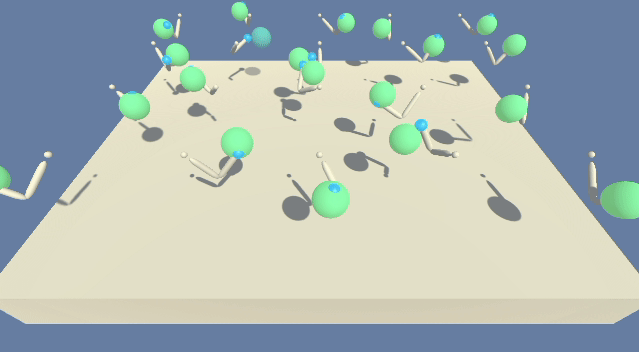
\includegraphics[width=0.75\linewidth]{images/example-env-image.png}
	\caption{A snapshot of the continuous control Unity-ML Reacher environment. White arms are agent-controlled (20 independent agents shown here), aiming to contain the blue hand in the green target locations.}
	\label{fig:example-game-image}
\end{figure}

\FloatBarrier

For the purposes of this project, the environment is considered solved when a 100-episode average of +30 is reached. That is, the average score over 100 concurrent episodes during training is above +30 reward from moving the arm appropriately.

\section{Approach}

The overall approach used herein was to utilize the \textit{Deep Deterministic Policy Gradient} (DDPG) algorithm. This algorithm is explained in more detail in the following section.

\subsection{DDPG}

This algorithm is an actor-critic algorithm that adapts Q-learning for a continuous action space, wherein both a Q-function approximation is learned alongside a serially adapted policy. Similar to the DQN algorithm \cite{dqn}, target networks are utilized in learning both an \textit{actor} network and a \textit{critic} network drawing from experiences in an expanding experience replay buffer.

Here, the \textit{actor} network is responsible for leveraging the approximation of the Q-function to determine an optimal action per time step. In this specific instance, the Q-function is represented not as a tabular matrix, due to the continuous nature and under the assumption that the Q-function is differentiable, instead the actions are selected as a continuous maxima on the Q and utilize gradient ascent.

\begin{equation}
	\mathop{\mathbb{\text{max}}}_\theta\mathop{\mathbb{E}}_{s\sim D}\left[Q_{\phi}\left(s, \mu_{\theta}(s)\right)\right]
\end{equation}

Additionally, the \textit{critic} network is only concerned with improving the Q-function approximation, whereby the network evaluates the value of taken actions against the value of predicted actions suggested by the \textit{actor} network. This is very similar from the DQN algorithm, and thus follows a valuation from:

\begin{equation}
	Q^*(s, a) = \mathop{\mathbb{E}}_{s' \sim P}\left[r(s, a) + \gamma\mathop{\mathbb{\text{max}}}_{a'}Q^*(s', a')\right]
\end{equation}
for evaluating a Q-function utilizing the Bellman equation for capturing reward and current max estimations on states and actions from the \textit{critic} and \textit{actor} networks.

Finally, a unique addition to the DDPG algorithm in comparison to other deep network algorithms for handling exploration vs. exploitation regards how noise is introduced to action values. The standard DDPG algorithm utilized \textit{Ornstein-Uhlenbeck} noise processes \cite{ddpg}, which is a mean-regressing noise process that results in a dampening normal noise over a time period. Specifically, over each training episode the noise injected to action values are slowly dampened over an episode to revert to noise generated around a tight Gaussian with mean 0.

\subsection{Implementation}

The specific implementation of DDPG completed in this work took two major forms, one to implement the standard DDPG algorithm as detaile din \cite{ddpg}, and another that adapts this to learn from multiple agents in parallel using a shared experience replay buffer.

The former involves the following characteristics:
\begin{itemize}
	\item both \textit{actor} and \textit{critic} networks utilized a baseline and target network pairing during training, where target networks are updated using a per-step soft-update schedule with ratio $\tau$,
	\item the \textit{actor} network seemed to benefit from a simpler architecture in comparison to the \textit{critic} network,
	\item using a repeatable update schedule per step (i.e., the networks can be updated \textit{m} times per step) along with learning rate $\alpha$,
\end{itemize}

 \FloatBarrier
 
 Using these implementation details on top of the DDPG algorithm, I settled on the following hyperparameters:
 
 \FloatBarrier
 
 \begin{table}[!ht]
 	\centering
 	\begin{tabular}{ c | p{6cm} | c }
 		\textbf{hyperparameter} & \textbf{utility} & \textbf{value} \\
 		\hline
 		$\alpha$ & learning rate & $0.001$ \\
 		$\tau$ & target network soft-update rate & $0.001$ \\
 		$\gamma$ & discount factor on future returns & $0.99$ \\
 		$t\ update$ & number of steps to take before updating networks & $1$ \\
 		$num\ updates$ & number of updates to complete each time networks are updated during training & $2$ \\
 		$\mu$ & regression mean for Ornstein-Uhlenbeck noise & $0.0$ \\
 		$\theta$ & factor for weighing the delta of value from mean & $0.15$ \\
 		$\sigma$ & factor for weighing the Weiner (Gaussian) noise process & $0.2$ \\
 		\hline
 	\end{tabular}
 	\caption{Hyperparameters experimented with to train an agent using DQN.}
 	\label{tbl:parameters}
 \end{table}
 
 Values were either determined experimentally, such as by varying learning rate $\alpha$, $\tau$, $\gamma$, and the integers for the update schedule, or utilized from the original DDPG paper \cite{ddpg} as in the parameters for the noise process $\mu$, $\theta$, and $\sigma$.
 
 Lastly, different variations on architecture were tested, with major architectural changes primarily affecting the bound of steady-state long-term performance of the agents. For best results, it appeared that a two hidden layer \textit{actor} network and a two to three layer \textit{critic} network produced fairly stable results. Architectures are outlined below in Figure \ref{fig:nn-architecture}.
  
 \FloatBarrier
 
 \begin{figure}[!ht]
 	\centering
 	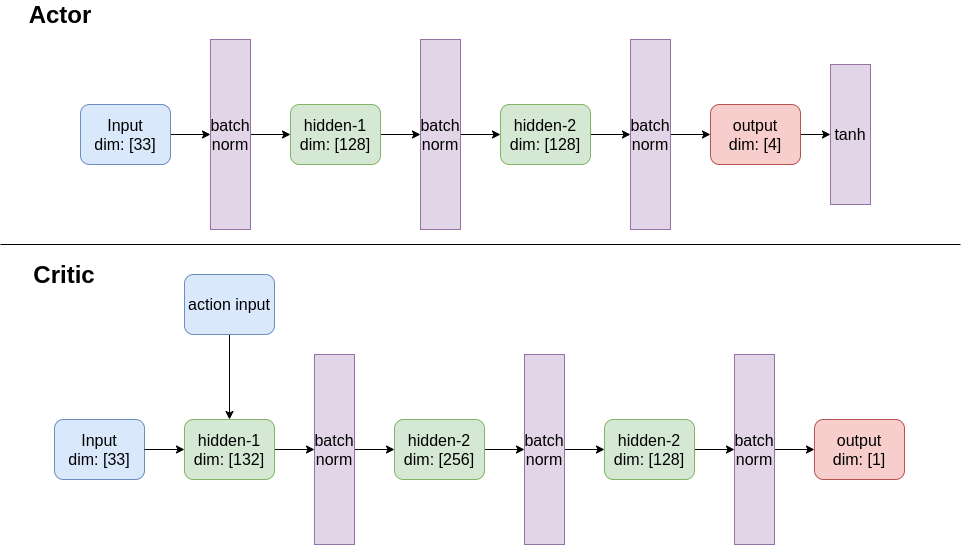
\includegraphics[width=0.8\linewidth]{images/architectures.png}
 	\caption{The architectures used in the final \textit{actor} and \textit{critic} networks in the DDPG algorithm. Though not specified, all activation functions are ReLU unless otherwise noted.}
 	\label{fig:nn-architecture}
 \end{figure}
 
 \FloatBarrier
 

\section{Results and Discussion}

\subsection{Learning Performance}

After determining an optimal set of parameters by running hyperparameter search on $\alpha \in \{0.0001, 0.001, 0.05\}$ and determining stable architectures for hidden layers across both \textit{actor} and \textit{critic} networks, the following results show training performance over a maximum 500 episode training session on different major versions of experiments.

\FloatBarrier

\begin{figure}[!ht]
	\centering
	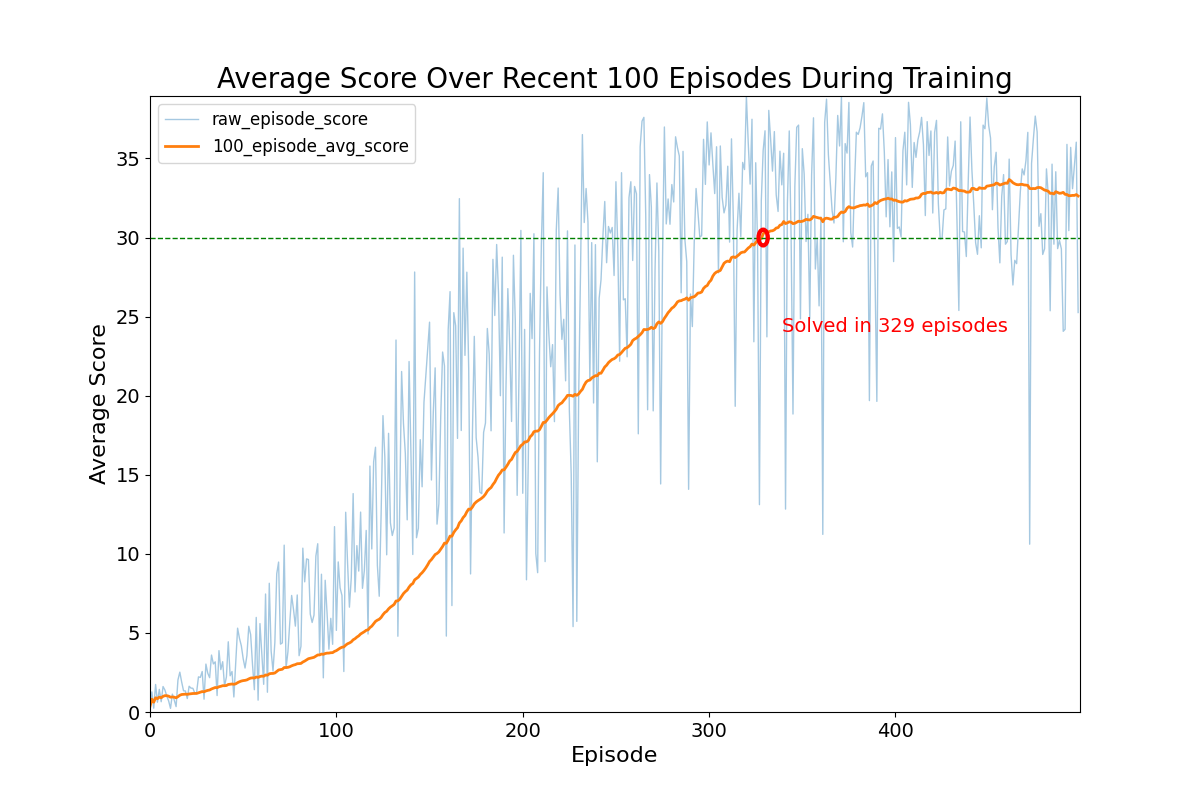
\includegraphics[width=0.75\linewidth]{images/ddpg-single-results.png}
	\caption{Per episode and 100-episode average score for an agent trained using the single agent environment. Here, $num\ updates$ was set to 10 to account for slower replay buffer cycling of a single agent. With the single arm, the agent was able to learn to achieve a 100-episode average score of +30 over 329 episodes of training.}
	\label{fig:ddpg-single-results}
\end{figure}

\FloatBarrier

The results in Figure \ref{fig:ddpg-single-results} illustrate the ability of the DDPG algorithm to learn to solve the Reacher environment in 329 episodes when leveraging experiences from a single training arm. I also aimed to investigate whether utilizing the 20-agent version of the Reacher environment would enable the DDPG algorithm (with some minor adaptations to how it extract experiences from the replay buffer) to learn more quickly and more stably from interactions in the environment. Specifically, notice that although the average seems fairly stable across learning, reaching a ceiling of approximately ~+35 reward on average, there seems to be quite a bit of fluctuation in per-episode performance. Some episodes still show scores of +12 reward, for instance, which suggests that training on and averaging across a single agent shows some variance in terms of performance. As Figure \ref{fig:ddpg-multi-results} illustrates, this was successfully remedied by extending DDPG to the multi-agent training environment.

\FloatBarrier

\begin{figure}[!ht]
	\centering
	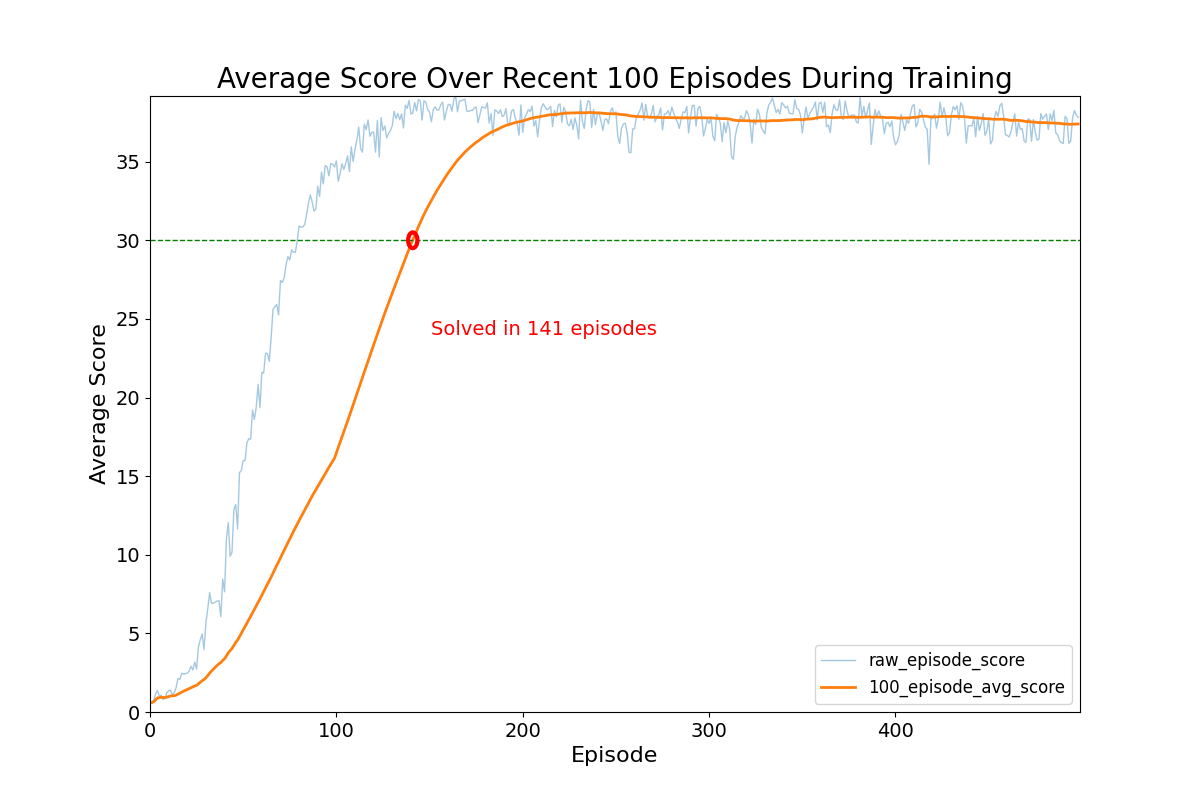
\includegraphics[width=0.75\linewidth]{images/ddpg-multi-results.png}
	\caption{Per episode and 100-episode average score for agents trained using the 20-agent environment. Here, $num\ updates$ was set to 2 to account for more rapid replay buffer cycling due to multiple agents sending experience tuples per step. In this condition, agents were able to on average achieve a 100-episode mean score of +30 over 141 episodes of training.}
	\label{fig:ddpg-multi-results}
\end{figure}

\FloatBarrier

The results shown in Figure \ref{fig:ddpg-multi-results} show that the multi-agent environment greatly improves training performance, achieving a 100-episode average of +30 in only 141 episodes of training. Not only that, but the long-term performance ceiling of this set of agents also stabilizes at approximately +37, again improving upon training on a single agent environment. This may be due to a few reasons, for instance the ability to leverage experiences from different agents in a shared experience replay buffer more quickly cycles through possible experiences each agent could see, since many state-action combinations could be observed before even arriving in a precursor state through their own experiences. Additionally, stability is greatly improved due to the fact that though experiences are pooled in a single replay buffer, each agent is learning independently, so the variability observed in Figure \ref{fig:ddpg-single-results} are averaged out across all of the learning agents.

\subsubsection{Final Architecture Results}

Though results presented earlier are quite strong, the baseline DDPG algorithm also utilizes batch normalization for each layer in the \textit{actor} network and each \textit{critic} network layer following concatenation of state input with action input (see Figure \ref{fig:nn-architecture}). This was deemed to be the required in the final architecture for the solution in this project, thus the final results in Figure \ref{fig:ddpg-multi-batch-results} show the slight benefit of having these normalization layers between hidden layers in the networks.

\FloatBarrier

\begin{figure}[!ht]
	\centering
	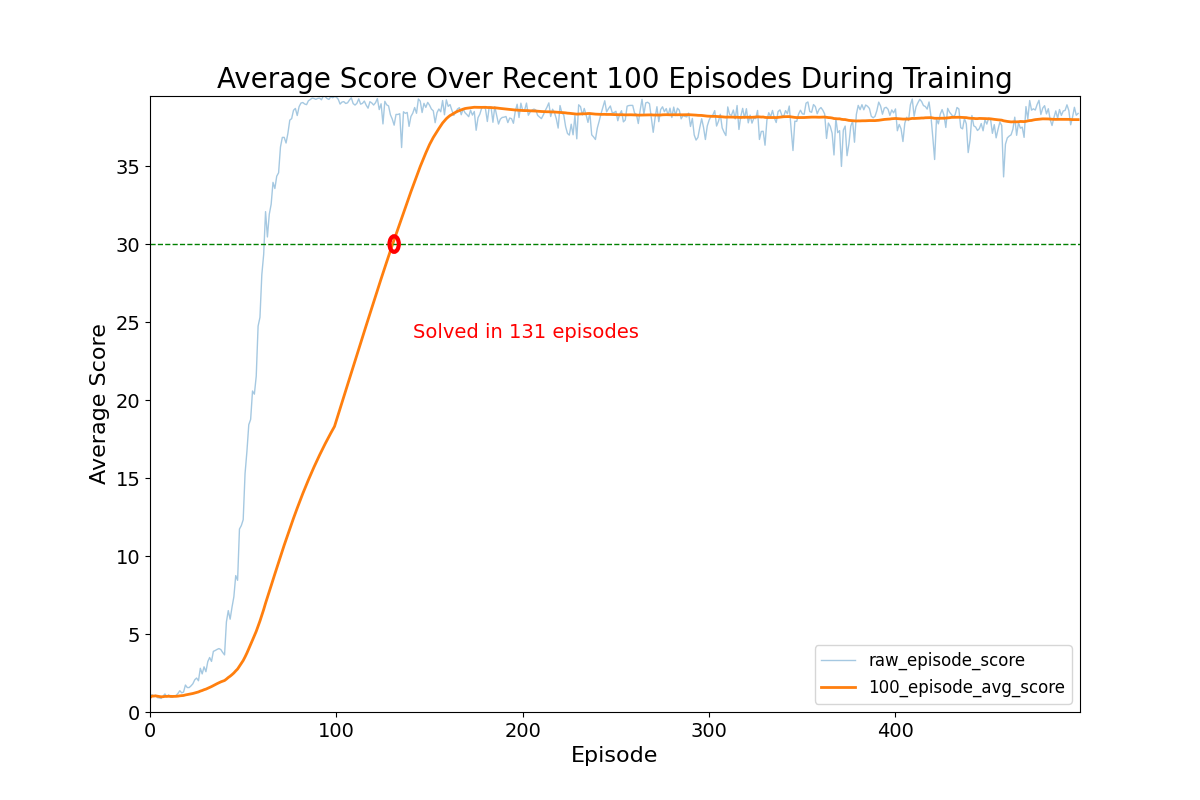
\includegraphics[width=0.9\linewidth]{images/ddpg-multi-batch-results.png}
	\caption{Per episode and 100-episode average score for agents trained using the 20-agent environment using batch normalization layers in \textit{actor} and \textit{critic} networks. Here, $num\ updates$ was set to 2 to account for more rapid replay buffer cycling due to multiple agents sending experience tuples per step. In this condition, agents were able to on average achieve a 100-episode mean score of +30 over 131 episodes of training.}
	\label{fig:ddpg-multi-batch-results}
\end{figure}

\FloatBarrier

These results show that DDPG, using batch normalization layers on a 20-agent environment results in the most stable, rapid training in the Reacher environment. This result even further improved the results of the multi-agent training results observed in Figure \ref{fig:ddpg-multi-results} since this not only maintains scale of data on forward passes in the network, but also inherently assists with regularizing the network throughout training \cite{batch}. This suggests that batch normalization assists in model training since deviations from optimality and any bias towards overfitting is mitigated all throughout the training process.


\subsection{Next Steps}

Some obvious next steps were to complete an intended comparison of DDPG to other multi-agent potential algorithms such as PPO or D4PG. This is obvious given that the DDPG algorithm was able to best perform when extended to capitalizing on the multi-agent environment to facilitate generating a shared experience replay buffer but yet maintain 20 individual instances of the agents.

Some next steps that were thought of to possibly introduce improvement if experimented with appropriately included:
\begin{itemize}
	\item experimenting with different noise processes, specifically examining how effective an explicit Gaussian noise process would be or by determining if a decay factor for noise over training episodes would improve long-term performance,
	\item experimenting with different parameters for the Ornstein-Uhlenbeck noise process, particularly for $\theta$ and $\sigma$ for controlling the variance of injected noise,
	\item determining if any variations to activation functions (aside from the $tanh$ used in \textit{actor} network output since this assists in bounding action values) in both \textit{actor} and \textit{critic} networks could change the effectiveness of training, particularly to help speed up training by still capturing non-deterministic qualities of the policy and Q-function approximations but enabling more course assessments of deviations from true values,
	\item further experimenting with the idea of introducing differences between the \textit{actor} and \textit{critic} networks, thereby introducing more fine-tuned abilities of the networks to capitalize on more quickly learning a policy by learning from actions and values somewhat independently,
	\item some variation of the evaluation system used in the \textit{critic} network that may incorporate a more advantage-based system as in the extension from DQN to duelling DQN \cite{duelling}.
\end{itemize}

Given that the DDPG algorithm has seen extensive use and extensions to achieve better performance and/or to work more directly with multi-agent environments with interaction (e.g., D4PG), this also remains the most logical next step for achieving improvement on the existing DDPG algorithm presented herein.

\section{Conclusion}

In conclusion, an agent was able to be trained using the DDPG algorithm in order to learn how to move an imaginary arm such that it maintains specific target positions over time. It appears that learning from the experiences of multiple agents was positively beneficial for the algorithm, which begs the idea that implementing a multi-agent algorithm for this multi-agent Reacher environment may better capitalize on cross-agent learning. Even this this being said, some minor improvements may be possible on the baseline implementation of DDPG presented herein, where noise processes and more experimentation with architectures may have exposed the potential for better training and long-term generalized performance.

\bibliographystyle{unsrt}
\bibliography{refs}
% \begin{thebibliography}{9}
% \bibitem{littman}
% Leslie~Pack Kaelbling, Michael~L Littman, and Andrew~W Moore.
% \newblock Reinforcement learning: A survey.
% \newblock {\em Journal of artificial intelligence research}, 4:237--285, 1996.
% \end{thebibliography}

\end{document}
